\documentclass{article}
\usepackage{eecstex}
\usepackage{pgfplots}

\title{EE 120 HW 03}
\author{Bryan Ngo}
\date{2021-02-10}

\begin{document}

\maketitle

\section{LTI Statements}

\begin{enumerate}
    \item False, consider the system \(y[n] = nx[n]\). This is causal, but is not bounded by some \(B_x\).
    \item True, this means that \(h[n]\) is absolutely integrable, or \(\sum_{k \in \Z} |h[n]| = \sum_{k \in [i, j]} |h[n]| = B_x\), where \(i, j\) are the bounds of the impulse response.
    \item True, this means that \(h(t)\) is not absolutely integrable, since the absolute value means that we are integrating strictly positive values over all of \(\R\).
    \item False, consider \(h[n] = 1\), then \(\sum_{k \in \Z} h[k]\) diverges.
    \item True % justify this one
\end{enumerate}

\section{Impulse Response of Discrete Time LTI Systems}

\subsection{}

\begin{equation}
    h[n] = \alpha^n u[n]
\end{equation}
\textbf{Stability}:
\begin{equation}
    \sum_{k \in \Z} \alpha^k u[k] = \sum_{k \geqslant 0} \alpha^k = \frac{1}{1 - \alpha}
\end{equation}
\textbf{Causality}: The system is causal since \(h[n] = 0\) for \(n < 0\).

\subsection{}

\begin{equation}
    h[n] = \beta^n u[3 - n]
\end{equation}
\textbf{Stability}:
\begin{equation}
    \sum_{k \in \Z} \beta^k u[3 - k] = \sum_{k \leqslant 3} \beta^k = \sum_{k \in [0, 2]} \beta^k + \sum_{k \geqslant 0} \left(\frac{1}{\beta}\right)^k = 1 + \beta + \beta^2 + \frac{1}{1 - \frac{1}{\beta}}
\end{equation}
\textbf{Causality}: The system is \emph{not} causal since \(h[n] \neq 0\) for \(n = -1\), for example.

\subsection{}

\begin{equation}
    h[n] = n (0.6)^n u[n]
\end{equation}
\textbf{Stability}:
\begin{equation}
    \sum_{k \in \Z} k (0.6)^k u[k] = \sum_{k \geqslant 0} k (0.6)^k
\end{equation}
Observe that the series converges. \\ % TODO: how?
\textbf{Causality}: The system is causal since \(h[n] = 0\) for \(n < 0\), for example.

\subsection{}

\begin{equation}
    h[n] = u[n] - u[n + 100]
\end{equation}
\textbf{Stability}: Note that this is a flipped rectangle function shifted to the domain \([-100, 0]\), meaning that its \(\sum_{k \in \Z} |h[k]| = 100\). \\
\textbf{Causality}: The system is \emph{not} causal since \(h[n] = -1\) for \(n \in [-100, 0]\).

\section{Impulse Response of Continuous Time LTI systems}

\subsection{}

\begin{equation}
    h(t) = e^{-3t} u(t - 5)
\end{equation}
\textbf{Stability}: The integral is
\begin{equation}
    \int_{\R} |h(t)| \, dt = \int_5^\infty e^{-3t} \, dt = \left.-\frac{1}{3} e^{-3t}\right|_5^\infty = \frac{e^{-15}}{3}
\end{equation}
\textbf{Causality}: The system is causal since \(h(t) = 0\) for \(t < 5\).

\subsection{}

\begin{equation}
    h(t) = e^{-4t} u(3 - t)
\end{equation}
\textbf{Stability}: The integral is
\begin{equation}
    \int_{\R} |h(t)| \, dt = \int_{-\infty}^3 e^{-4t} \, dt = \left.-\frac{1}{4} e^{-4t}\right|_{-\infty}^3
\end{equation}
which diverges. \\
\textbf{Causality}: The system is \emph{not} causal since \(h(t) = e^4\) for \(t = -1\).

\subsection{}

\begin{equation}
    h(t) = e^{-4|t|}
\end{equation}
\textbf{Stability}: The integral is
\begin{align}
    \int_{\R} e^{-4|t|} \, dt &= \int_{-\infty}^0 e^{4t} \, dt + \int_0^\infty e^{-4t} \, dt \\
    &= 2 \int_0^\infty e^{-4t} \, dt = \left.-\frac{1}{2} e^{-4t}\right|_0^\infty = \frac{1}{2}
\end{align}
\textbf{Causality}: The system is \emph{not} causal since \(h(t) = e^{-4}\) for \(t = -1\).

\subsection{}

\begin{equation}
    h(t) = t e^{-t} u(t)
\end{equation}
\textbf{Stability}: The integral is
\begin{align}
    \int_{\R} |h(t)| \, dt = \int_0^\infty t e^{-t} \, dt = \left.-(t + 1) e^{-t}\right|_0^\infty = 1
\end{align}
\textbf{Causality}: The system is causal since \(h(t) = 0\) for \(t < 0\).

\section{LTI System Impulse Response}

\begin{align}
    h_1[n] &= \sin[8n] \\
    h_2[n] &= a^n u[n] \\
    x[n] &= \delta[n] - a \delta[n - 1]
\end{align}
By the properties of convolution,
\begin{equation}
    y[n] = (h_2[n] \ast h_1[n]) \ast x[n]
\end{equation}
Finding what \((h_2 \ast x)[n]\) is,
\begin{align}
    a^n u[n] \ast (\delta[n] - a\delta[n - 1]) = a^n u[n] - a^{n - 1} a u[n - 1] = a^n (u[n] - u[n - 1]) = a^n \delta[n] = \delta[n]
\end{align}
where we can eliminate the exponential term because the function is only nonzero at \(n = 0\), so \(a^0 = 1\).
Then, finding the final convolution,
\begin{equation}
    \delta[n] \ast \sin[8n] = \sin[8n]
\end{equation}

\section{Manual Convolution}

\subsection{}

\begin{equation}
    (x + w) \ast y = (x \ast y) + (w \ast y)
\end{equation}
Plotting \((x + w) \ast y\),
\begin{center}
    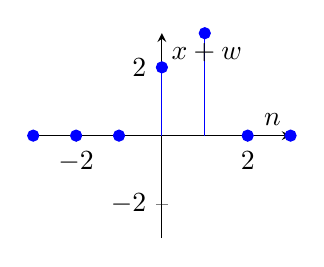
\begin{tikzpicture}
        \begin{axis}[
            xlabel=\(n\), ylabel={\(x + w\)},
            axis lines=middle,
            ymin=-3, ymax=3,
            width=0.4\textwidth
        ]
        \addplot[
            ycomb,
            color=blue,
            mark=*
        ]
        coordinates {
            (-3, 0)
            (-2, 0)
            (-1, 0)
            (0, 2)
            (1, 3)
            (2, 0)
            (3, 0)
        };
        \end{axis}
    \end{tikzpicture}
    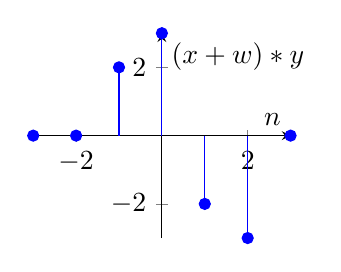
\begin{tikzpicture}
        \begin{axis}[
            xlabel=\(n\), ylabel={\((x + w) \ast y\)},
            axis lines=middle,
            ymin=-3, ymax=3,
            width=0.4\textwidth
        ]
        \addplot[
            ycomb,
            color=blue,
            mark=*
        ]
        coordinates {
            (-3, 0)
            (-2, 0)
            (-1, 2)
            (0, 3)
            (1, -2)
            (2, -3)
            (3, 0)
        };
        \end{axis}
    \end{tikzpicture}
\end{center}
Likewise, plotting \(x \ast y\) and \(w \ast y\),
\begin{center}
    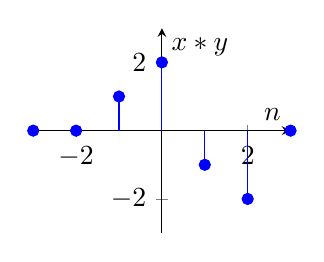
\begin{tikzpicture}
        \begin{axis}[
            xlabel=\(n\), ylabel={\(x \ast y\)},
            axis lines=middle,
            ymin=-3, ymax=3,
            width=0.4\textwidth
        ]
        \addplot[
            ycomb,
            color=blue,
            mark=*
        ]
        coordinates {
            (-3, 0)
            (-2, 0)
            (-1, 1)
            (0, 2)
            (1, -1)
            (2, -2)
            (3, 0)
        };
        \end{axis}
    \end{tikzpicture}
    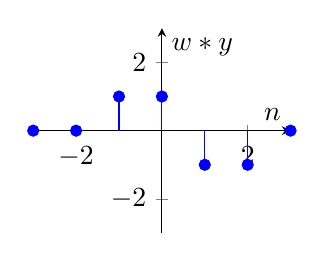
\begin{tikzpicture}
        \begin{axis}[
            xlabel=\(n\), ylabel={\(w \ast y\)},
            axis lines=middle,
            ymin=-3, ymax=3,
            width=0.4\textwidth
        ]
        \addplot[
            ycomb,
            color=blue,
            mark=*
        ]
        coordinates {
            (-3, 0)
            (-2, 0)
            (-1, 1)
            (0, 1)
            (1, -1)
            (2, -1)
            (3, 0)
        };
        \end{axis}
    \end{tikzpicture}
\end{center}
As observed, their sum is equal to the above plot, so the distributive property holds.

\subsection{}

\begin{equation}
    (x \ast y) \cdot w \neq x \ast (y \cdot w)
\end{equation}
Drawing these two plots,
\begin{center}
    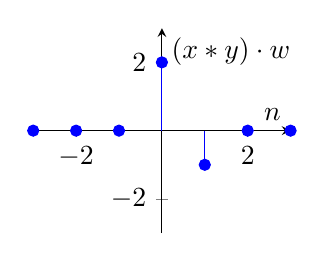
\begin{tikzpicture}
        \begin{axis}[
            xlabel=\(n\), ylabel={\((x \ast y) \cdot w\)},
            axis lines=middle,
            ymin=-3, ymax=3,
            width=0.4\textwidth
        ]
        \addplot[
            ycomb,
            color=blue,
            mark=*
        ]
        coordinates {
            (-3, 0)
            (-2, 0)
            (-1, 0)
            (0, 2)
            (1, -1)
            (2, 0)
            (3, 0)
        };
        \end{axis}
    \end{tikzpicture}
    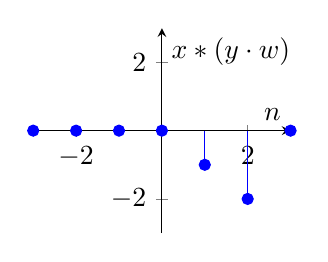
\begin{tikzpicture}
        \begin{axis}[
            xlabel=\(n\), ylabel={\(x \ast (y \cdot w)\)},
            axis lines=middle,
            ymin=-3, ymax=3,
            width=0.4\textwidth
        ]
        \addplot[
            ycomb,
            color=blue,
            mark=*
        ]
        coordinates {
            (-3, 0)
            (-2, 0)
            (-1, 0)
            (0, 0)
            (1, -1)
            (2, -2)
            (3, 0)
        };
        \end{axis}
    \end{tikzpicture}
\end{center}
which are clearly not equal.

\section{Convolution \& Correlation}

\begin{align}
    x(t) &=
    \begin{cases}
        2 & t \in (0, 3) \\
        0 & \text{elsewhere}
    \end{cases} \\
    g(t) &= e^{-\frac{t}{2}} u(t)
\end{align}

\subsection{}

\begin{align}
    x(t) \ast g(t) &= \int_{\R} x(\tau) e^{-\frac{1}{2} (t - \tau)} u(t - \tau) \, d\tau \\
    &= \int_0^3 2e^{-\frac{1}{2} (t - \tau)} u(t - \tau) \, d\tau \\
    &= \int_t^{t - 3} -2e^{-\frac{v}{2}} u(v) \, dv \\
\end{align}

\section{Convolution Practice}

\end{document}
